\documentclass[10pt]{amsart}
\usepackage{amssymb,latexsym,amsmath}
\usepackage{tikz-cd}
\usepackage{pgf,tikz}
\usetikzlibrary{arrows}
\usetikzlibrary{shapes.geometric}
\usetikzlibrary{positioning}
\usetikzlibrary{calc}
\usetikzlibrary{decorations.markings}
\usetikzlibrary{backgrounds}
\usepackage{xcolor}

\begin{document}

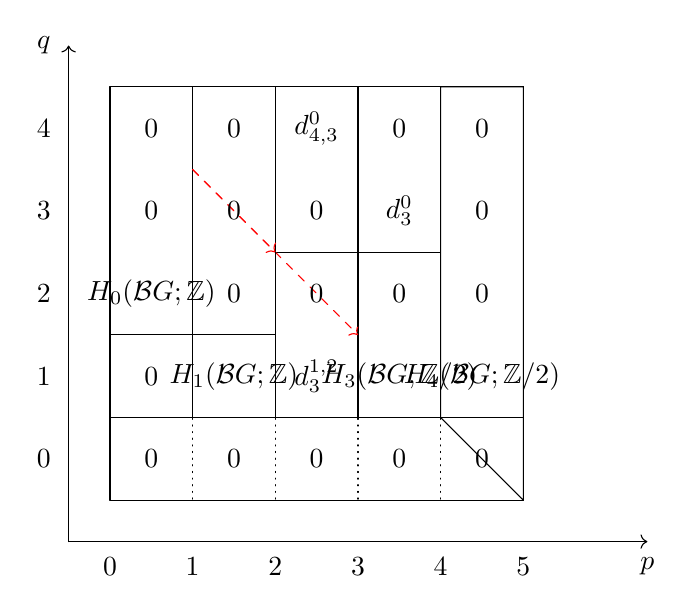
\begin{tikzpicture}[line cap=round,line join=round,x=0.7cm,y=0.7cm,scale = 1.5]

\draw [->] (-0.5,-0.5) -- (-0.5,5.5);
\draw [->] (-0.5,-0.5) -- (6.5,-0.5);

% Labels of the y-axis
\node at (-0.8,5.5) {$q$};
\node at (-0.8,4.5) {4};
\node at (-0.8,3.5) {3};
\node at (-0.8,2.5) {2};
\node at (-0.8,1.5) {1};
\node at (-0.8,0.5) {0};

% Labels of the x-axis
\node at (6.5,-0.8) {$p$};
\node at (0,-0.8) {0};
\node at (1,-0.8) {1};
\node at (2,-0.8) {2};
\node at (3,-0.8) {3};
\node at (4,-0.8) {4};
\node at (5,-0.8) {5};

% Drawing the boxes
\draw (0,0)--(0,5)--(5,5)--(5,0)--cycle;
\draw (0,1)--(0,2)--(1,2)--(1,5)--(5,5)--(5,1)--cycle;
\draw (1,1)--(1,2)--(2,2)--(2,5)--(5,5)--(5,1)--cycle;
\draw (2,1)--(2,3)--(3,3)--(3,5)--(5,5)--(5,1)--cycle;
\draw (3,1)--(3,3)--(4,3)--(4,5)--(5,5)--(5,1)--cycle;
\draw (4,1)--(4,5)--(5,5)--(5,0)--cycle;

% Drawing the horizontal arrows
\draw[red,dashed,->] (1,4)--(3,2);
\draw[red,dashed,->] (1,4)--(2,3);

% Drawing the vertical arrows
\draw[dotted] (1,3)--(1,0);
\draw[dotted] (2,3)--(2,0);
\draw[dotted] (3,3)--(3,0);
\draw[dotted] (4,3)--(4,0);
\draw[dotted] (5,3)--(5,0);

% Labelling the boxes
\node at (0.5,0.5) {$0$};
\node at (0.5,1.5) {$0$};
\node at (0.5,2.5) {$H_{0}(\mathcal{B}G;\mathbb{Z})$};
\node at (0.5,3.5) {$0$};
\node at (0.5,4.5) {$0$};

\node at (1.5,0.5) {$0$};
\node at (1.5,1.5) {$H_{1}(\mathcal{B}G;\mathbb{Z})$};
\node at (1.5,2.5) {$0$};
\node at (1.5,3.5) {$0$};
\node at (1.5,4.5) {$0$};

\node at (2.5,0.5) {$0$};
\node at (2.5,1.5) {$d_{3}^{1,2}$};
\node at (2.5,2.5) {$0$};
\node at (2.5,3.5) {$0$};
\node at (2.5,4.5) {$d_{4,3}^{0}$};

\node at (3.5,0.5) {$0$};
\node at (3.5,1.5) {$H_{3}(\mathcal{B}G;\mathbb{Z}/2)$};
\node at (3.5,2.5) {$0$};
\node at (3.5,3.5) {$d_{3}^{0}$};
\node at (3.5,4.5) {$0$};

\node at (4.5,0.5) {$0$};
\node at (4.5,1.5) {$H_{4}(\mathcal{B}G;\mathbb{Z}/2)$};
\node at (4.5,2.5) {$0$};
\node at (4.5,3.5) {$0$};
\node at (4.5,4.5) {$0$};

\end{tikzpicture}

\end{document}